\documentclass[../mit-general-chemistry.tex]{subfiles}
\begin{document}



\chapter{Periodic table}






\section{Photoelectron spectroscopy}


In X-ray photoelectron spectroscopy (PES) we revisit the photoelectric
effect. PES is a technique to measure the energy levels of the
orbitals of atoms.

If we hit an atom with a photon with enough incident energy, $E_i$,
we'll get a free electron with a kinetic energy $E_k = E_i -
\text{IE}$. This gives us the ionization energies (work functions) of
the atom (remember that $E_{\Psi} = -\text{IE}$ from earlier).

\begin{align*}
  \overbrace{E}^{\text{X-ray photon}} + \ce{Ne} &\rightarrow\ce{Ne+} + \overbrace{e^-}^{\text{+ kinetic energy}} \\
  1s^22s^22p^6 &\rightarrow 1s^22s^22p^5 + e^-\\
\end{align*}

In this case we say that it is one of the outermost electrons that are
ejected, but this is only because of the energy of the photon. Had we
put in enough energy, we could have ejected any of the electrons of
the atom. This would also have had an impact on the resulting kinetic
energy of the ejected electron which is the difference between the
energy of the photon and the ionization energy of that orbital.

We use X-rays for PES as they have higher frequency, and thus higher
energy, than UV-light, so as to make sure we eject all the electrons
of the atom we study.

As we know that the kinetic energy of the ejected electron is equal to
the difference between the incident energy of the photon and the
ionization/binding energy of the electron/orbital.


\begin{example}
  Suppose we hit some neon gas atom with a photon with $E_i =
  1254\si{\eV}$ and we detect an ejected electron with $E_k = 1232
  \si{\eV}$. What is the ionization energy of the orbital that
  electron came out of?

  It is an easy subtraction. We calculate
  \begin{equation*}
    \text{IE} = E_i - E_k = 1254 - 1232 = 22 \si{\eV}
  \end{equation*}
\end{example}

Continuing to hit the neon atom we get the energy levels for all the
orbitals of the atom.

\begin{center}
  \begin{tabular}{lll}
    \toprule
    shell ($n$)& IE (\si{\eV})& $E_k (\si{\eV})$ \\
    \midrule
    $2p$ & 22 & 1232 \\
    $2s$ & 48 & 1206 \\
    $1s$ & 780 & 384 \\
    \bottomrule
  \end{tabular}
\end{center}
\begin{marginfigure}
  \begin{center}
    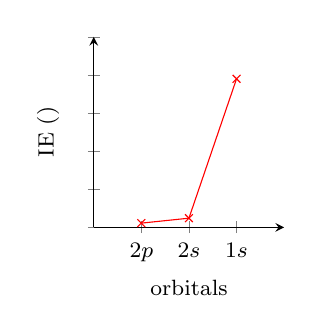
\begin{tikzpicture}[
        font={\footnotesize}
      ]
      \begin{axis}[
          width=4cm,
          height=4cm,
          xmin=0,
          xmax=4,
          ymin=0,
          ymax=1000,
          axis lines = left,
          domain = 0:3,
          xlabel = orbitals,
          ylabel = IE (\si{\eV}),
          xtick = {1, 2, 3},
          xticklabels = {$2p$, $2s$, $1s$},
          %ytick = {0, 5000, 10000},
          yticklabels = \empty,
          clip = false,
        ]
        \addplot[color=red,mark=x] coordinates {
          (1, 22)
          (2, 48)
          (3, 780)
	};
      \end{axis}
    \end{tikzpicture}
  \end{center}
  \captionof{figure}{Energy levels of the atomic orbitals of neon. \label{fig:neo:IE}}
\end{marginfigure}


There is a significant difference between the energy levels of the
{\em valence electron} orbitals ($s2$ and $p2$) and the energy lavel
of the orbital of the {\em core electrons}.

The orbital energy levels in multi-electron atoms depend on the two
quantum numbers $n$ and $l$. That is why we assume that $p_x$, $p_z$
and $p_y$ all have the same energy level.


\begin{example}
  If a certain element was studied under x-ray PES displays an
  emission spectrum with five distinct kinetic energies, what are all
  of the possible elements that this could be?

  First, we know that this is an element that have five energy levels
  and corresponding orbitals. The first five orbitals are $1s, 2s, 2p,
  3s, 3p$ so the elements are in the first three periods of the
  periodic system.

  Second, ``our element'' is an element that have electrons in the
  $3p$-orbital. The elements that fits that description are
  \ce{Al, Si, P, S, Cl, Ar}. So that is our answer.

  Had we known the exact wavelengths of the emission lines or the
  incident and kinetic energies we would have been able to say exactly
  what element it is that emits those lines.
\end{example}














\section{Periodic trends of the periodic table}



The periodic table was compiled in 1869 by Dmitri Mendeleev. In 1869,
only 60-70\% of the elements we know today were discovered. In the
periodic table, elements were grouped by their properties that he saw
(e.g. Group 1: \ce{Li, Na, K}: soft, reactive metals; Group 18:
\ce{He, Ne, Ar}: inert gases, they do not react).

Today, we look at the electron configuration and see that \ce{Li, Na,
  K} have {\em one valence electron in a $s$ state} whereas \ce{He,
  Ne, Ar} have filled shells.

The lonely valence of the Group 1 elements is the explanation to why
they are so reactive: they are so willing to give up that electron.



\subsection{Ionization energy}

Ionization energy (IE) is the minimum energy required to remove an
electron form an atom.

It is assumed that we mean the {\em first ionization energy} unless
otherwise specified.

\begin{equation}
  \text{IE} = E_{nl}
\end{equation}


Consider the ionization of boron, \ce{{}_5B}.

\begin{align*}
  \ce{B}(1s^22s^22p^1) &\rightarrow \ce{B+}(1s^22s^2) + e^-
  & \deltaE = E_p - E_r = \text{IE} = -E_{2p}
\end{align*}

This was the first ionization energy, yaking an electron from the
atomic orbital of the highest energy level.

Lets consider the second ionization energy

\begin{align*}
  \ce{B+}(1s^22s^2) &\rightarrow \ce{B^2+}(1s^22s^1) + e^-
  & \deltaE = \text{IE}_2 = -E_{2s} ~\text{in}~\ce{B+}
\end{align*}



Now, consider the energy required to remove an electron from \ce{B}
compared to \ce{B+}.

\begin{align*}
  \ce{B+ &-> B^2+ + e_{2s}^- } & \deltaE = \text{IE}_2 = -E_{2s} ~\text{in}~\ce{B+}\\
  \ce{B &-> B+ + e_{2s}^- } & \deltaE = \text{IE}_{2s} = -E_{2s} ~\text{in}~\ce{B}\\
\end{align*}

These two ionization energies are not going to be of the same
size. The electron in the ion is less shielded from it's nucleus and
therefore feel a stronger attractive force and hence it is going to
require more force to remove the electron from the atom.



\subsubsection{Periodic trends in ionization energy}

As we go across a row, ionization energy increases. As we go across
a row $Z$ increases while $n$ remains the same. This increases \Zeff.


As we go down a column, or group, ionization energy decreases. As we go down a
column $Z$ increases but so does $n$. We need to consider three things
\begin{itemize}
\item $Z$ is increasing
\item the distance between the outermost electron and the nucleus is
  increasing
\item there are even more shielding from an increasing amount of other
  electrons
\end{itemize}

It turns out that the ionization energy decreases down a column or
down a group.


These trends are generally true but not one hundred percent. We can
see some deviation. Looking at the second period, we see ``glitches''
to the general trend between beryllium and boron as well as between
nitrogen and oxygen.

\begin{center}
  \begin{tikzpicture}[
      font={\footnotesize}
    ]
    \begin{axis}[
        full,
        title={Ionization energy for the second period},
        width=.9\textwidth,
        height=4cm,
        xmin=0,
        xmax=9,
        ymin=400,
        ymax=2100,
        axis lines = left,
        domain = 0:3,
        xlabel = elements,
        ylabel = IE (\si{\kilo\joule\per\mol}),
        xtick = {1, 2, 3, 4, 5, 6, 7, 8},
        xticklabels = {\ce{Li}, \ce{Be}, \ce{B}, \ce{C}, \ce{N}, \ce{O}, \ce{F}, \ce{Ne}},
        %ytick = {0, 5000, 10000},
        %yticklabels = \empty,
        clip = false,
      ]
      \addplot[color=red,mark=x] coordinates {
        (1, 520)
        (2, 900)
        (3, 800)
        (4, 1090)
        (5, 1400)
        (6, 1310)
        (7, 1680)
        (8, 2080)
      };
    \end{axis}
  \end{tikzpicture}
\end{center}

The ``glitch'' between nitrogen and oxygen show us that
\begin{equation*}
  \text{IE}_{\ce{B}} < \text{IE}_{\ce{Be}}
\end{equation*}

We also show the electron configuration of the two elements.

\begin{center}
  \begin{MOdiagram}[names,labels,labels-fs=\footnotesize]
    \atom[Be]{left}{
      1s = {0.5; pair},
      2s = {2; pair},
      2p = {3; },
    }
    \atom[B]{right}{
      1s = {0.5; pair},
      2s = {2; pair},
      2p = {3; up},
    }
    \EnergyAxis[title=$E$]
  \end{MOdiagram}
\end{center}



Looking at the electron configurations for beryllium and boron below,
we can see that the outermost electron of boron is that lonely
$2p$-orbital electron n entire energy level away which outweighs the
extra proton on the nucleus. That is on the next energy level which makes it
that easier to remove than one of the more negative $2s$-electrons.


Looking at nitrogen and oxygen in the chart above we see that
\begin{equation*}
  \text{IE}_{\ce{O}} < \text{IE}_{\ce{N}}
\end{equation*}
which also deviates from our general trend.

Looking at these energy level diagrams, we see that from nitrogen to
oxygen we start double up in the $2p$-subshells. This causes some
electron repulsion between the $2p_x$-electrons of oxygen and this is
the explanation of the trend glitch.

\begin{center}
  \begin{MOdiagram}[names,labels,labels-fs=\footnotesize]
    \atom[N]{left}{
      1s = {0.5; pair},
      2s = {1.5; pair},
      2p = {3; up, up, up},
    }
    \atom[O]{right}{
      1s = {0.5; pair},
      2s = {1.5; pair},
      2p = {3; pair, up, up},
    }
    \EnergyAxis[title=$E$]
  \end{MOdiagram}
\end{center}



Both of these phenomenon reoccurs in other periods as well.







\subsection{Electron affinity}



Electron affinity, \Eea, is the ability of an atom, or ion, to gain an
electron.

\ceeqstar{X + e^- -> X-}

Looking on this reaction with chlorine
\begin{align*}
  \ce{Cl + e^- &-> Cl-} & \deltaE = -349~\si{\kilo\joule\per\mol}
\end{align*}
we see that energy is released which means that \ce{Cl-} is actually
lower in energy than chlorine and this means that the ion is more
stable than the neutral atom is.

We measure electron affinity as
\begin{equation*}
  \Eea = - \deltaE\quad\text{from the reaction}
\end{equation*}

\Eea = \SI{349}{\kilo\joule\per\mol} is a very large electron affinity
and this tells us that chlorine very easily gains an electron to form
\ce{Cl-}. Chlorine actually has one one of the largest electron
affinities.

Electron affinity can be either positive or negative (unlike
ionization energy which can only be positive).

We look at a reaction where the electron affinity is negative:
\begin{align*}
  \ce{N + e^- &-> N-} &\deltaE = +7~\si{\kilo\joule\per\mol} \\
  &&\Eea = -7~\si{\kilo\joule\per\mol} \\
\end{align*}

We see that $\Eea < 0$ and this means we need to put that amount of
energy into the reaction to make it happen, this is not a favorable
reaction. Thos means that nitrogen has low electron affinity, it will
not easily gain an electron. This also tells us that the \ce{N-}-ion
is less stable than the neutral atom.


\subsubsection{Trends in electron affinity}

We see a similar trend in electron affinity as we did in ionization
energy. Electron affinity increases as we go along a row (period) in
the periodic system.

Electron affinity decreases as we go down a column (group) in the
periodic system. The noble gases have a negative electron affinity
which makes sense since they have full outer shells and are considered
inert. Halogens have the highest electron affinity.






\subsection{Electronegativity}


Electronegativity ($\chi$) is the ability of an atom to attract an electron
density from another atom.

It turns at that
\begin{equation*}
  \chi \propto \frac{1}{2}(\Eea + \text{IE})
\end{equation*}


\subsubsection{Trends in the periodic system}


Since $\chi \propto \frac{1}{2}(\Eea + \text{IE})$, if we take the
periodic system and divide it up in quadrants. In the upper, right
quadrant we have high electron affinity and high ionization energy so
we will also have high electronegativity.

In the lower, left corner we have the opposite conditions and
therefore also a low electronegativity.

Elements with a high electronegativity are electron
acceptors. Elements with a low electronegativity are electron donors.

The common measurment of electronegativity is not the one above but
the Pauling numbers. They do however share the same trends as the
definition above.






\subsection{Atomic radius}

When we talk about atomic radius we essentially talk about atomic
size. One way to think of the atomic radius is a radius $r$ within
which 90\% of the electron density is contained.

Another way is to measure the distance between two adjacent nuclei of
the same element, $d$, and divide that with 2
\begin{equation*}
  r = \frac{1}{2}d
\end{equation*}

The two model of thinking do however come up with similar numbers for
atom size.

Atomic radius for the elements decrease as we go across a period as
\Zeff increases.

Atomic radius increases as we go down columns (groups) of the periodic
system since we are adding electrons further and further away from the
nucleus.











\section{Isoelectronic atoms and ions}



Isoelectronic atoms and ions are species with the same electron
configuration.

Consider neon with electron configuration $1s^22s^2p^6$ other atoms
can not have this configuration but ions can. Consider

\begin{equation*}
  \underbrace{\ce{N^3-} \ce{O^2-} \ce{F-}}_{\text{larger radius than neutral parent}}
  \ce{Ne}
  \underbrace{\ce{Na+} \ce{Mg^2+} \ce{Al^3+} \ce{S^4+}}_{\text{smaller atomic radius than neutral parent}}
\end{equation*}

The atomic radii of anions increases as the put on new electrons. The
atomic radii of cations decreases as they lose electrons but also as
remaining electrons fell a stronger \Zeff due to loss of shielding.





\addsec{Summary}
\end{document}
